\documentclass[titlepage,article,paper=b4,twocolumn]{jlreq}
\setlength{\columnseprule}{0.5pt}
\setlength{\columnsep}{5\zw}
\usepackage[top=30mm,bottom=20mm,left=15mm,right=15mm]{geometry}
\usepackage{amssymb,mathtools,mathcomp}
\usepackage{enumitem,tasks}
\usepackage{physics,physics2}
\settasks{label-width=2\zw}
\usephysicsmodule{ab,ab.braket}
\usepackage{bm}
\usepackage{graphicx,tabularx,here}
\usepackage{tikz,tikz-3dplot}
\usetikzlibrary{math,angles,quotes,calc,intersections}
\usepackage{kyotsutest}
\usepackage{answerbox}
\usepackage[pdftitle={中３数学１学期期末問題},pdfauthor={まさし},hidelinks]{hyperref}
\newcommand{\Div}{\mathbin{\textrm{\textdiv}}}

\NewPageStyle{examQ}
{nombre_position=top-left,
nombre={\Large{$\smash{\raisebox{-0.5\zh}{\href{https://fanme.link/@masashi\_00\_}{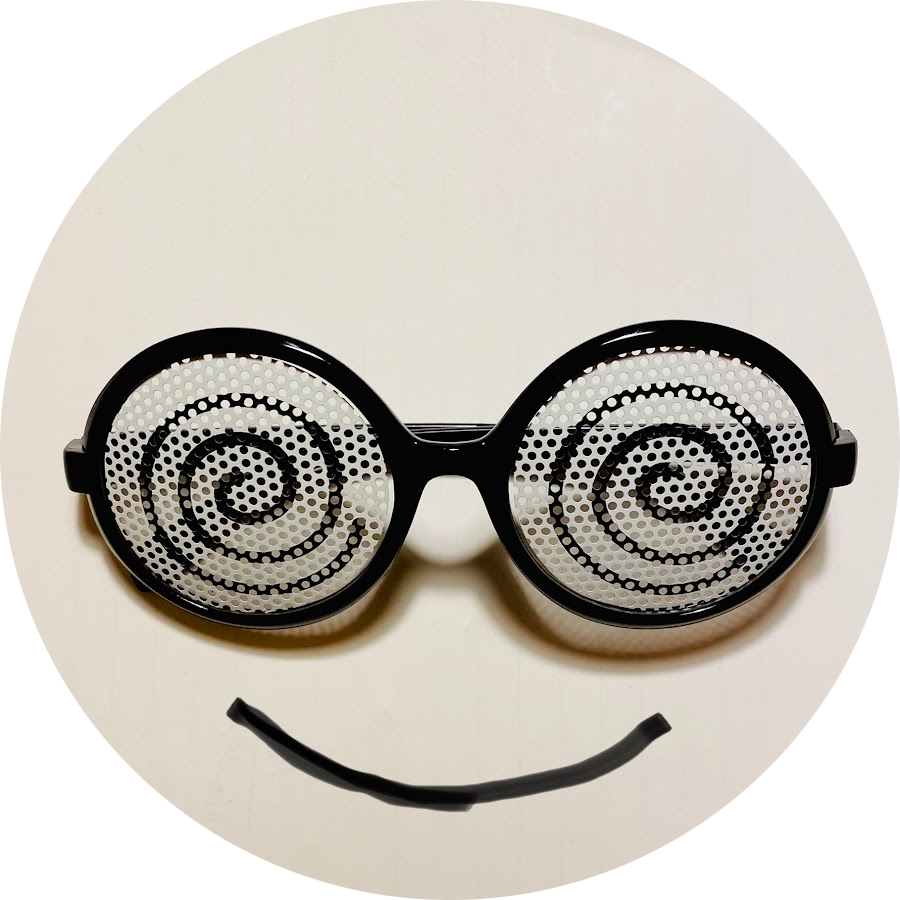
\includegraphics[width=2\zw]{../../common/icon-masashi.png}}}}$ 中学３年 数学 １学期期末対策 問題用紙\quad\textrm{No.~\thepage}}},
running_head_position=top-right,
odd_running_head=\normalsize{\textrm{３年\underline{\hspace{2\zw}}組\underline{\hspace{2\zw}}番
\hspace{0.5\zw}氏名\underline{\hspace{15\zw}}}}}
\NewPageStyle{examA}
{nombre_position=top-left,
nombre={\Large{$\smash{\raisebox{-0.5\zh}{\href{https://fanme.link/@masashi\_00\_}{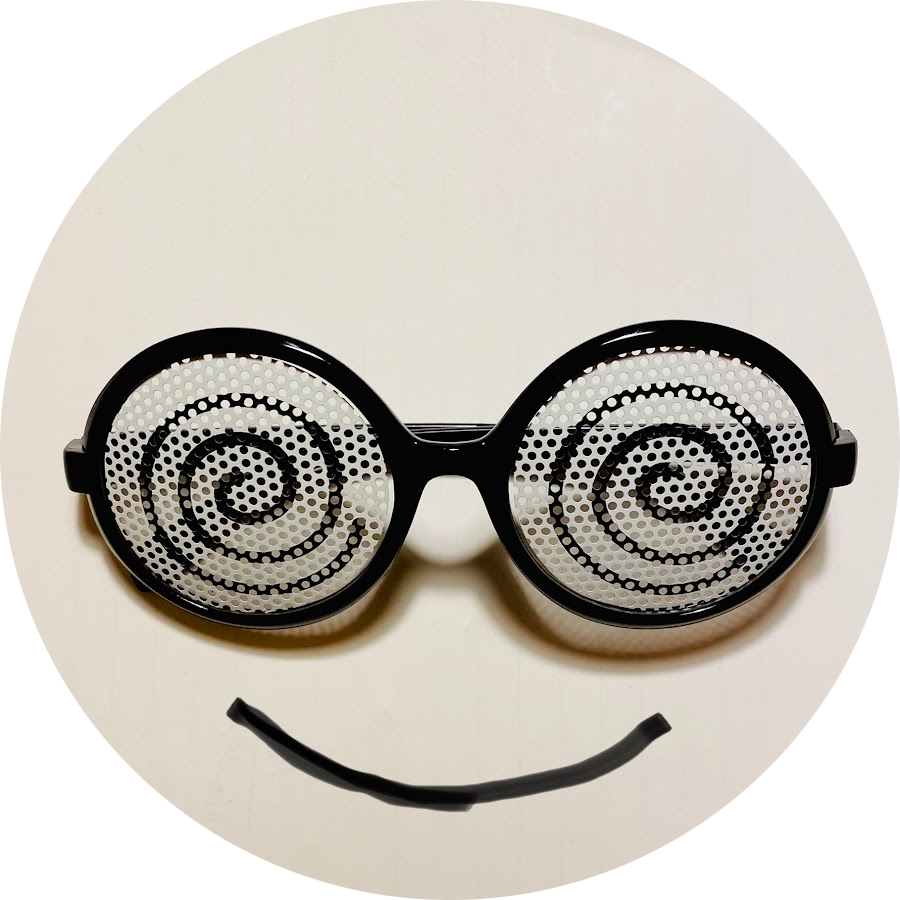
\includegraphics[width=2\zw]{../../common/icon-masashi.png}}}}$ 中学３年 数学 １学期期末対策 解答用紙\quad\textrm{No.~\thepage}}},
running_head_position=top-right,
odd_running_head=\normalsize{\textrm{３年\underline{\hspace{2\zw}}組\underline{\hspace{2\zw}}番
\hspace{0.5\zw}氏名\underline{\hspace{15\zw}}}}}

\begin{document}
\pagestyle{examQ}
\setcounter{page}{1}
\begin{enumerate}[label=\arabic*.]
\setlength{\labelsep}{\zw}
%1
\item 次の数の平方根を求めなさい。
\vspace{5mm}
\begin{tasks}[label=(\arabic*)](3)
\task $4$
\vspace{5mm}

\task $11$
\vspace{5mm}

\task $0.16$
\vspace{5mm}

\task $\dfrac{25}{49}$
\vspace{5mm}

\task $\sqrt{25}$
\vspace{5mm}
\end{tasks}
\vfill


%2
\item 次の数を，根号を使わずに表しなさい。
\vspace{5mm}
\begin{tasks}[label=(\arabic*)](3)
\task $\sqrt{36}$
\vspace{5mm}

\task $-\sqrt{49}$
\vspace{5mm}

\task $\sqrt{\ab(-11)^{2}}$
\vspace{5mm}
\end{tasks}
\vfill


%3
\item 次の式を計算しなさい。
\vspace{5mm}
\begin{tasks}[label=(\arabic*)](2)
\task $\sqrt{2} \times \sqrt{6}$
\vspace{5mm}

\task $\sqrt{45} \times \sqrt{72}$
\vspace{5mm}

\task $\sqrt{54} \Div \sqrt{18}$
\vspace{5mm}

\task $6\sqrt{2} \Div 2\sqrt{6}$
\vspace{5mm}

\task $\sqrt{147} - \sqrt{27} - \sqrt{48}$
\vspace{5mm}

\task $\dfrac{3}{\sqrt{2}} + \sqrt{18} - \dfrac{5}{\sqrt{50}}$
\vspace{5mm}
\end{tasks}

\begin{tasks}[resume,label=(\arabic*)](1)
\task $2\ab(\sqrt{3} + 3\sqrt{2}) - \ab(4\sqrt{3} - \sqrt{2})$
\vspace{5mm}
\end{tasks}
\vfill


%4
\item 次の方程式を解きなさい。
\vspace{5mm}

\begin{tasks}[label=(\arabic*)](2)
\task $5{x}^{2} - 30 = 0$
\vspace{5mm}

\task ${x}^{2} + 11x = 0$
\vspace{5mm}

\task ${x}^{2} + x - 56 = 0$
\vspace{5mm}

\task ${x}^{2} + 6x + 9 = 0$
\vspace{5mm}

\task $9{x}^{2} - 4x - 1 = 0$
\vspace{5mm}

\task $\ab(3x - 1)\ab(2x + 5) = -12$
\vspace{5mm}
\end{tasks}

\begin{tasks}[resume,label=(\arabic*)](1)
\task $\ab(3x - 1)^{2} + \ab(3x - 1) - 110 = 0$
\vspace{5mm}
\end{tasks}
\vfill\vfill
\newpage


%5
\item 次の文が正しければ{\maru}を，間違っていれば{\batsu}を書きなさい。
\begin{enumerate}[label=(\arabic*)]
\setlength{\labelsep}{\zw}
\item $9$の平方根は$3$である。
\vspace{5mm}
\item $0.01$の平方根は，$0.1$と$-0.1$である。
\vspace{5mm}
\item $0$の平方根は$0$である。
\vspace{5mm}
\item $\sqrt{100}$は$\pm 10$である。
\vspace{5mm}
\item $\sqrt{-64}$は$-8$である。
\vspace{5mm}
\end{enumerate}
\vfill


%6
\item 次の問いに答えなさい。
\begin{enumerate}[label=(\arabic*)]
\setlength{\labelsep}{\zw}
\item $x = 11$，$y = -6$ のとき，${x}^{2} + 2xy + {y}^{2}$ の値を求めなさい。
\vspace{5mm}
\item $x + y = 5$，$xy = -3$ のとき，${x}^{2} + {y}^{2}$ の値を求めなさい。
\vspace{5mm}
\item $1$以上$20$以下の素数をすべて書きなさい。
\vspace{5mm}
\end{enumerate}
\vfill


%7
\item 次の問いに答えなさい。
\begin{enumerate}[label=(\arabic*)]
\setlength{\labelsep}{\zw}
\item $\sqrt{17} < n < \sqrt{39}$ となるような自然数$n$を，すべて求めなさい。
\vspace{5mm}
\item $\sqrt{11 - n}$ が整数となるような自然数$n$を，すべて求めなさい。
\vspace{5mm}
\item $\sqrt{98n}$ が整数となるような自然数$n$のうち，最も小さいものを求めなさい。
\vspace{5mm}
\end{enumerate}
\vfill


%8
\item 2次方程式 ${x}^{2} + ax - \ab(3a + 13) = 0$ の解の1つが $x = 2$ であるとき，
$a$の値を求めなさい。また，他の解も求めなさい。
\vspace{5mm}
\vfill


%9
\item ある自然数に$4$を加えて$2$乗すると，もとの数よりも$60$大きくなった。
このとき，もとの数を求めなさい。
\vfill\vfill
\newpage


%10
\item 縦の長さが $26{\,}\textrm{m}$，横の長さが $35{\,}\textrm{m}$ の長方形の畑がある。
この畑に，下の図のように縦と横に同じ幅の道をつくり，
残った畑の面積が $850{\,}\textrm{m}^{2}$ となるようにする。
道の幅を何mにすればよいか，求めなさい。\vspace{5mm}

\begin{figure}[H]
\centering
\begin{tikzpicture}[x=7mm, y=7mm]\small
\begin{scope}
\draw[cap=round] (0,0) to [bend left=30] node[midway, fill=white] {$26{\,}\textrm{m}$} (0,5.2);
\draw[cap=round] (0,0) to [bend right=20] node[midway, fill=white] {$35{\,}\textrm{m}$} (7,0);
\clip (0,0) rectangle (7,5.2);
\fill[lightgray]  (0,0) rectangle (7,5.2);
\fill[white]  (4,0) rectangle (4.5,5.2) (0,3) rectangle (7,3.5);
\draw[gray] (0,0)rectangle(4,3)(4.5,0)rectangle(7,3)(0,3.5)rectangle(4,5.2)(4.5,3.5)rectangle(7,5.2);
\end{scope}
\draw (0,0)rectangle(7,5.2);
\end{tikzpicture}
\end{figure}
\vspace{5mm}
\vfill


%11
\item 半径 $r{\,}\textrm{m}$ の円形の土地の周囲に，幅 $a{\,}\textrm{m}$ の道がある。
この道の面積を $S{\,}\textrm{m}^{2}$，
道の真ん中を通る円周の長さを $\ell{\,}\textrm{m}$ とするとき，
$S = a\ell$ となることを証明しなさい。\vspace{5mm}

\begin{figure}[H]
\centering
\begin{tikzpicture}\small
\begin{scope}
\clip (0,0) circle (2.3);
\fill[lightgray]  (0,0) circle (2.3);
\draw[dashed] (0,0)circle(2);
\node[fill=lightgray] at (0,2) {$\ell{\,}\textrm{m}$};
\fill[white]  (0,0) circle (1.7);
\draw[gray] (0,0)circle(1.7);
\draw(0,0)--(5,0);
\draw[cap=round] (0,0) to [bend left=30] node[midway, fill=white] {$r{\,}\textrm{m}$} (1.7,0)
(1.7,0) to [bend left=45] (2.3,0);
\end{scope}
\draw (0,0)circle(2.3);
\draw[cap=round] (2.16,0.1) to [bend left=20] (2.5,0.5) node[above right, inner xsep=0.5mm, inner ysep=0]{$a{\,}\textrm{m}$};
\end{tikzpicture}
\end{figure}
\vspace{5mm}
\vfill\vfill
\newpage


%12
\item 連続する3つの整数のうち，
最小の数の平方と最大の数の平方の和から$2$を引いた数が，
中央の数の平方の$2$倍に等しいことを証明しなさい。
\vspace{5mm}
\vfill\vfill
\newpage
\end{enumerate}

\newpage

\pagestyle{examA}
\setcounter{page}{1}

\begin{ansbox}
\pbox[3]{5}
\end{ansbox}

\begin{ansbox}
\pbox{3}
\end{ansbox}

\begin{ansbox}
\pbox[2]{7}
\end{ansbox}

\begin{ansbox}
\pbox[2]{7}
\end{ansbox}

\begin{ansbox}
\pbox{5}
\end{ansbox}

\begin{ansbox}
\pbox{2}
\pbox{1}
\end{ansbox}

\begin{ansbox}
\pbox[1]{3}
\ptxt{1}{l}{\quad$n ={}$}
\ptxt{2}{l}{\quad$n ={}$}
\ptxt{3}{l}{\quad$n ={}$}
\end{ansbox}

\begin{ansbox}
\pbox*{2}
\ptxt{1}{l}{\quad$a ={}$}
\ptxt{2}{l}{\quad 他の解：\ $x ={}$}
\end{ansbox}

\begin{ansbox}
\pbox*[3]{1}
\end{ansbox}

\begin{ansbox}
\pbox*[3]{1}
\ptxt{1}{r}{$\textrm{m}$\hspace{\zw}}
\end{ansbox}
\newpage

\begin{ansbox}[height=120mm]
\pbox*{1}
\end{ansbox}

\begin{ansbox}[height=90mm]
\pbox*{1}
\end{ansbox}
\newpage
\end{document}